\chapter{Introducción y objetivos}
\label{cap:introduccion}

En la actualidad, la empresa BQ se ha especializado en fabricar y distribuir impresoras 3D junto con sus consumibles. En 2013, se creó un departamento de Innovación y Desarrollo, encabezado por Juan Gonzalez y Alberto Valero. En ese comienzo se distribuye material relacionado con las impresoras 3D para que cualquier persona pueda contruirse una impresora 3D. Este material no es fabricado por BQ directamente, tan solo realiza la tarea de distribuidor.\\

A medida que BQ adquiere experiencia en el mercado, empieza a crear una línea de investigación para desarrollar sus propias impresoras 3D, como es el caso de la impresora Witbox y la impresora Prusa Hephestos (ver Figura \ref{fig:impresoras_bq}). En este caso BQ tiene un papel importante a lo largo del desarrollo del producto, desde la elección de las características finales del mismo, así como el aspecto final del packaging, es decir, BQ pasa de tener un papel de distribuidor a ser la parte principal del desarrollo del producto.\\

\begin{figure}[h!]
    \centering
    \begin{subfigure}[b]{0.4\textwidth}
        \centering
        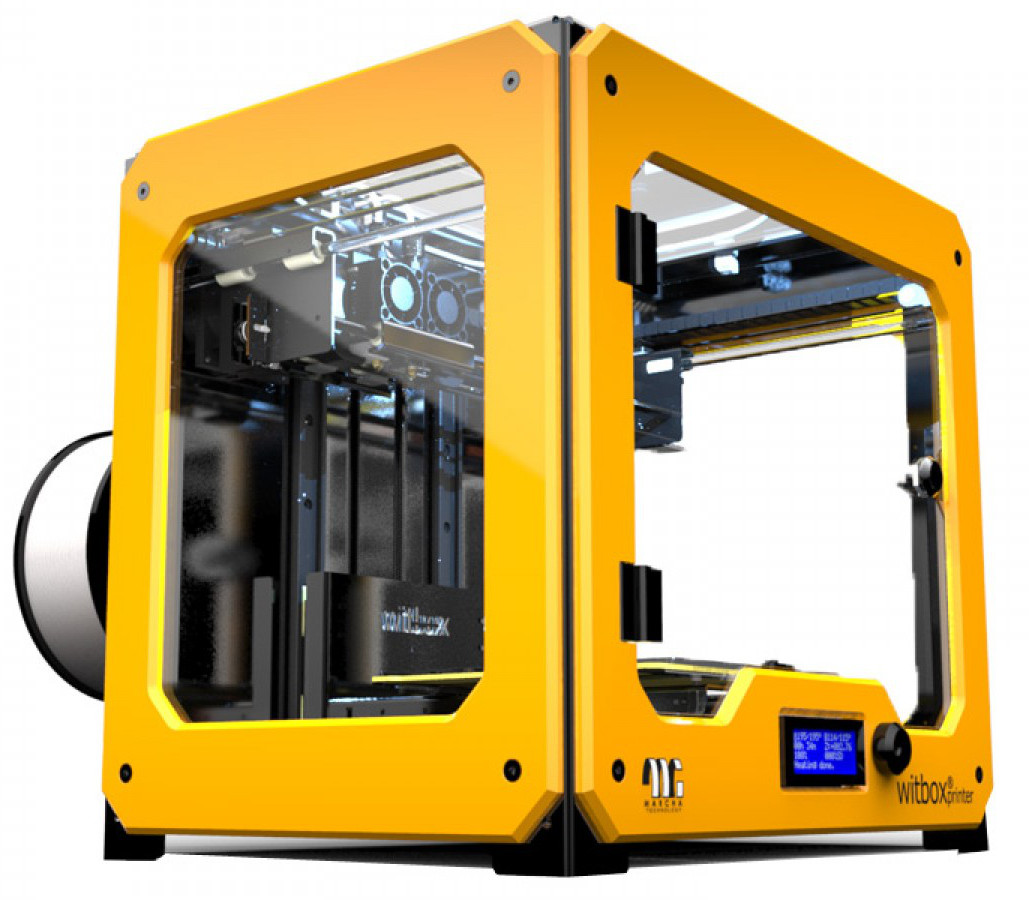
\includegraphics[width=\linewidth]{images/Witbox.jpg}
        \label{fig:estado_witbox}
    \end{subfigure}
    ~
    \begin{subfigure}[b]{0.3\textwidth}
        \centering
        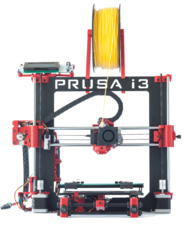
\includegraphics[width=\linewidth]{images/190px-HEPHESTOS.png}
        \label{fig:estado_hephestos}
    \end{subfigure}
    \caption[Impresoras fabricadas por BQ.]{Impresoras fabricadas por BQ. Podemos ver las dos impresoras que desarrolla BQ, a la izquierda, Witbox impresora que ya se vende montada. A la derecha, Prusa Hephestos, se vende en formato kit para que el usuario final la monte (DIY). Fuente \cite{bq}.}
    \label{fig:impresoras_bq}
\end{figure}

A la vez que se venden las impresoras 3D, BQ también vende el principal consumible para que las impresoras 3D puedan funcionar, plástico en forma de filamento. Este plástico se distribuye en unas bobinas (ver Figura \ref{fig:estado_filamento}), en las que está almacenado un hilo continuo de plástico con un diámetro específico, en este caso, $1.75mm$, así mismo, cada filamento tiene un color distinto. Este consumible, es creado por otras empresas y BQ simplemente distribuye. Una vez que BQ tiene un puesto en el mercado de las impresoras 3D, decide entonces crear su propio filamento y tener más controlado la calidad del filamento que vende.\\

\begin{figure}[h!]
    \centering
    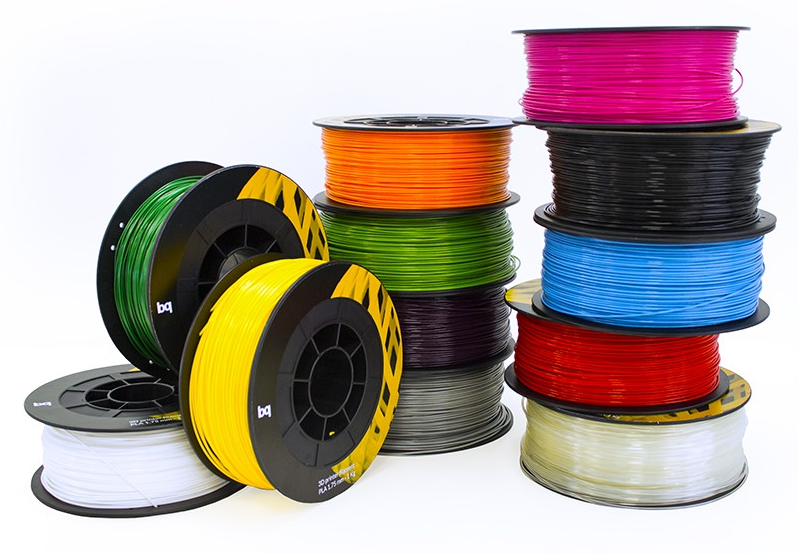
\includegraphics[width=0.5\textwidth]{images/filamento_bq.png}
    \caption[Distintos filamentos de BQ.]{Distintos filamentos de BQ. Fuente \cite{bq}.}
    \label{fig:estado_filamento}
\end{figure}

Sin embargo, la fabricación del filamento es más complicada que la construcción de las impresoras 3D. Se necesitan máquinas capaces de fundir plástico y darle la forma de filamento, estás máquinas son las extrusoras, de las cuales BQ no dispone ninguna y no se tiene previsión de que al comprar una se pueda llegar a amortizar su compra. Por ello, se decide sub-contratar el proceso de fabricación a una empresa experta en la extrusión de plásticos.\\

La empresa PESL es especialista en extrusión de perfilería de plástico. BQ y PESL empiezan a trabajar en la fabricación de un filamento que cumpla las características necesarias para las impresoras 3D. En una primera aproximación estas características son, el material y el diámetro final. Después de pruebas de fabricación del filamento por parte de ambas empresas, BQ empieza a vender filamento fabricado por PESL.\\

Aparte de vender el filamento que fabrica PESL, BQ también hace uso de él en sus instalaciones y desarrollo de proyectos, se empieza a detectar entonces un problema, no todas las bobinas del mismo lote de fabricación tienen la misma calidad, llegando a darse el caso que en una misma bobina, no todo el filamento es igual. Los problemas detectados tienen que ver con el aspecto visual del filamento, la mezcla de color no es homogénea, y provoca que se genere un degradado de color en las piezas impresas. Así mismo, y mucho más importante, el diámetro del filamento no es constante (ver Figura \ref{fig:muestra_filamento}).

\begin{figure}[h!]
    \centering
    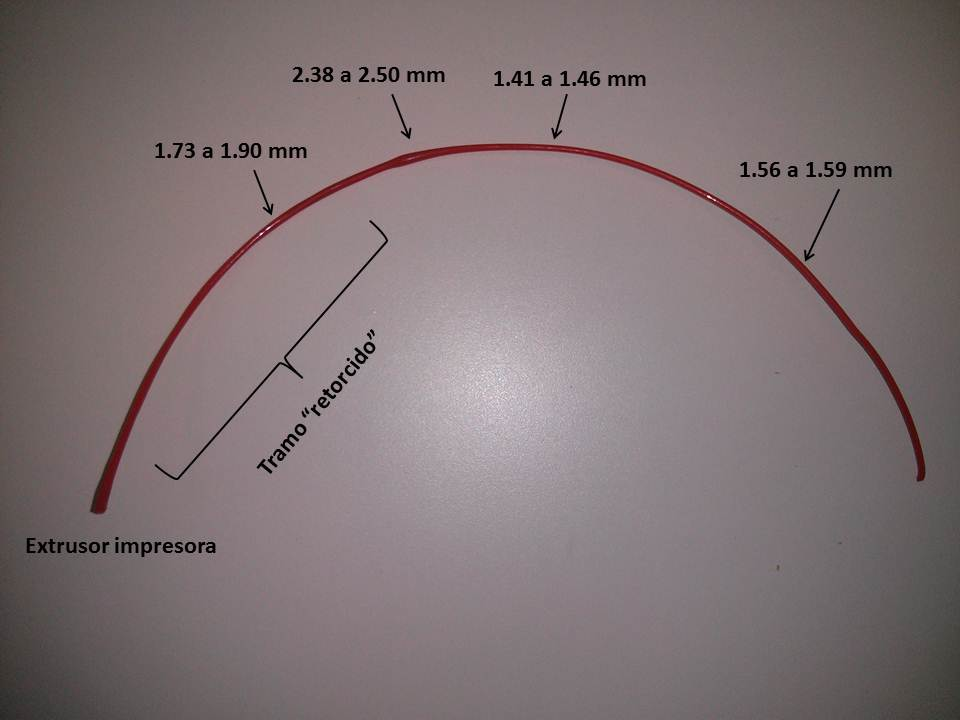
\includegraphics[width=0.6\textwidth]{images/atasco_rojo.jpg}
    \caption[Muestra de filamento con problemas en el diámetro]{Muestra de filamento con problemas en el diámetro. Podemos observar cómo en un tramo de filamento, el diámetro no es constante.}
    \label{fig:muestra_filamento}
\end{figure}

El problema que se tiene en el color, es algo secundario, ya que puede considerarse visual y no afecta al funcionamiento de los componentes de la impresora. No pasa lo mismo con el problema del diámetro, ya que la manera en la que se descubre, es que las impresoras dejan de imprimir pasado un tiempo, puesto que si el diámetro nominal del filamento sale de un determinado rango de valores, tanto por exceso como por déficit, se producen atascos en la impresora. Estos atascos, en el mejor de los casos, sólo supone la limpieza del extrusor de la impresora y se puede volver a utilizar, pero en ocasiones el atasco puede deja inservible el extrusor y es necesario reemplazarlo.\\

No tardan en llegar las primeras reclamaciones de clientes, en las que su impresora deja de imprimir de forma temporal o incluso que el uso del filamento de BQ daña las impresoras 3D de los clientes, suponiendo un gasto extra tanto para BQ, ya que ofrece una garantía por su producto, como para PESL, que no todo el filamento que fabrica reporta beneficios. Es por ello que se pone en aviso a PESL y se toman decisiones para mejorar este problema.\\

A pesar de que PESL es especialista en extrusión de perfilería de plástico, es la primera vez que se dedican a la extrusión de filamento. Aunque de forma teórica no hay ninguna diferencia, si lo hay en el uso final que se va a dar al plástico. En el caso de un perfil extruido, su uso será rematar obras, recubrimiento aislante y tuberías. El uso final que se le va a dar al filamento de plástico va a suponer un refundido del material, proceso en el cual influye la manera en cómo se fabricó. Igualmente el material con el que se trabaja para fabricar filamento, no es el mismo que el que se utiliza para extruir perfiles y requiere de otros tratamientos de fabricación.\\ 

Para minimizar estos problemas, se incorpora a la línea de fabricación un elemento mecánico, por el cual pasa el filamento, y si este supera un diámetro se parte y la producción es parada. También se empieza a registrar el diámetro del filamento y las temperaturas de fabricación en un ordenador para intentar tener un mejor control de la trazabilidad de las bobinas, y así acotar el problema que haya en la fabricación.\\

Tras estas mejoras, las reclamaciones de los clientes siguieron llegando a BQ y PESL y, con ellas, las pérdidas para ambos. Gracias a que cada bobina contiene un código QR en el que se incluye el número de lote de fabricación, se solicitan los registros del lote de fabricación a PESL para intentar ver posibles causas. Sin embargo, el tiempo desde que se piden hasta que son dados, es demasiado largo. Una vez que se tiene el registro, se comprueba que faltan datos de temperaturas, puesto que estos valores son introducidos a mano al no estar conectados con el ordenador que registra la información del diámetro. Y el muestreo de los datos no es siempre constante, por lo que hay tramos de la bobina de los que no se tienen información.\\

Desde BQ se decide entonces tomar una solución para tener todos los registros de una manera cómoda y fiable. Se piensa en desarrollar un sistema automático en el cual estén conectados todos los elementos que componen la línea de extrusión y así poder acceder a los datos de:

\begin{itemize}
    \item{Fecha de fabricación.}
    \item{Diámetro final del filamento.}
    \item{Temperaturas de todo el proceso.}
    \item{Velocidad de extrusión.}
\end{itemize}

Así mismo, esta información será almacenada en una base de datos, la cual se podrá acceder de manera remota. De esta manera, se quita carga de trabajo a PESL para que se dediquen a fabricar filamento, y desde BQ se puedan analizar los datos para ver causas de fallo.\\

El trabajo realizado para conseguir un primer demostrador de un sistema de adquisición de datos y comprobar que puede ser útil para solucionar el problema que tenemos, pasa por diferentes etapas en las que se encuentra buscar qué dispositivo es el más adecuado para llevar el control y, que este, sea estable, robusto y lo más versátil posible, para poder implementarlo en cualquier línea de extrusión. Una vez conseguido la unidad central de control, el siguiente paso será realizar la programación para que el sistema, de forma automática, adquiera los datos que se le indiquen y guarde la información en un medio físico para su posterior análisis.\\

Una vez que el sistema diseñado es capaz de almacenar la información, será necesario instalarlo en una línea de extrusión para demostrar que el sistema es válido ayudando a minimizar el error que se genera en la fabricación del filamento, y aumentar el porcentaje de bobinas con un filamento que cumpla los requisitos de calidad impuestos por BQ.

A continuación, se detallan los objetivos a conseguir en el proyecto:

\begin{itemize}
    \item Realizar un sistema capaz de leer la información más importante en la fabricación del filamento
    \item Instalar en una extrusora de filamento industrial.
    \item Estudio de los datos adquiridos y desarrollo del modelo teórico de la planta.
\end{itemize}
\label{Listado_objetivos}

\section{Organización de este documento}
\label{sec:organizacion}

En este primer capítulo hemos visto el problema que se presenta a la hora de obtener un filamento de calidad y la importancia de obtener una herramienta capaz de ayudarnos a entender cuales son las causas que provocan fallos durante la producción en la línea de extrusión. Vemos también la solución que se propone, realizar un sistema de adquisición de datos para el posterior análisis de los mismos.\\

En el Estado del arte se analizan las soluciones que otras empresas proponen para el mismo problema y cómo nuestro sistema puede mejorar los distintos sistemas disponibles en el mercado.\\

El capítulo 4, Desarrollo de la solución propuesta, muestra el trabajo realizado para cumplir el objetivo principal: Planificar las distintas tareas necesarias para el desarrollo del sistema, detallar las herramientas utilizadas y por qué se han decidido usar; y se verá la instalación del sistema en una línea de extrusión de pequeñas dimensiones, para poder comprobar como de válido es nuestro sistema\\

En Validación del sistema veremos los ensayos realizados para dar validez a que el sistema desarrollado es válido para minimizar el error presentado en la introducción del proyecto.\\

Por último, hablaremos de si el sistema desarrollado cumple el objetivo principal marcado. También veremos los aportaciones que se han derivado a la hora de realizar el proyecto, en forma de pequeños sistemas capaces de solucionar otros problemas que en un primer lugar no eran ámbito de este trabajo final de grado.\\